%!TEX root = ../main.tex
\begingroup
% \RedeclareSectionCommand[beforeskip=\chapteroneoffset]{chapter}
%%%%%%%%%%%%%%%%%%%%%%%%%%%%%%%
%%%%%%%%%%%%%%%%%%%%%%%%%%%%%%%
\chapter{Revitalization of the OLTC} % for Modern Grid Requirements}
\label{chap:intro}

% \begin{textblock*}{.7\textwidth}(70mm-\offset,25mm-\offset)%(70mm,25mm)
%     \begin{fquote}[Albert Einstein]
%         Two things are infinite: the universe and human stupidity; and I'm not sure about the universe.
%     \end{fquote}
% \end{textblock*}
\begin{textblock*}{.7\textwidth}(70mm-\offset,25mm-\offset)%(70mm,25mm)
    \begin{fquote}[William Stanley Jr.]
        The heart of the alternating current system.
    \end{fquote}
    % \begin{fquote}[Albert Einstein]
    %     For knowledge is limited to all we know and understand, while imagination embraces the entire world, and all there will be ever to know and understand.
    % \end{fquote}
\end{textblock*}

\endgroup

As first inventions regarding induction and induction coils were published in the early 19th century, nobody knew the impact these ideas could have.
The first developments and rivalry between power grid systems, \ac{DC} vs. \ac{AC}, was tending towards the latter side.
The use and spread of an \acs{AC} power system was enlarged by the transformer, making switching between different voltage levels seemless.
Long transmission lines were now facilitated through reducing losses under higher voltages. \quelle

This operational unit is still in heavy use today.
Later developments like the \ac{OLTC} enabled a variation in the transformer ratio under load, and therefore controlling load flows, compensate variations in voltage levels, or compensate currents in meshed grids. \autocite{schwab_2022}
Now, with the restructurization from centralized, machine dominated towards decentralized, small, and inverted-based electrical power generation, the transformer could be labelled outdated.
But the developments and ideas are ongoing like the invention of \textcite{maschinenfabrikreinhausengmbh_2023}.

Considering a combination of reliable and proven mechanical \acs{OLTC} transformers, with the dynamic capabilities of power electronics, their invention is targeting the faster dynamics of wind and solar generators, as well as flexible prosumers\footnote{often referred neologism coming from \glqq \textit{pro}active con\textit{sumers}\grqq}.
The added \ac{FSM} could help these units staying resilient to disturbances for a longer time, and therefore the grid to remain in a stable operational window. 

\newpage

\section{Research Interests}
\label{sec:research-interests}

A novel control method for this \acs{FSM} was developed by \cite{burlakin_2024}.
The transformer is connecting an off-shore wind farm with a sea cable to a \ac{PCC}.
Additionally, a \ac{VSC} is connected via a \acs{FSM} equipped transformer for compensation of the cable \autocite{burlakin_2024a}.
These control schemes are in the interest of this thesis, next to a developed power system simulation tool from the chair of electrical energy systems at the Friedrich-Alexander University Erlangen-Nuremberg \autocite{kordowich_2023}.
The tool is called \textit{diffpssi}, based on Python and the package \textit{PyTorch}, and with that allowing for model parameter optimizations.

The main idea is the extension of this power system simulation model with a capable variable ratio transformer.
Additionally, a standard discrete \acs{OLTC} controller is implemented, supplemented by the control scheme for the \acs{FSM}.
The capabilities of this improved \acs{FSM} module and its new control shall be investigated and compared to the standard \acs{OLTC} control.
As the central application of tap changing transformers is voltage support and indirect voltage stability enhancement \autocite{kundur_2022,milano_2010}, the comparisons are taken from this side.
With this background, folling main research question can be formulated for this thesis.

% \commenting{
%     \begin{itemize}[nosep]
%         \item Influence of OLTC control on possible operational uses: Short-term voltage stability, long-term voltage stability; 
%         \item Can a increased dynamic regulation help machine recovery?
%         \item Does the increased tap ratio gradient harm transient stability of machines?
%         Does it help or harm CCT of machines or machine groups?
%         \item Transformers act as big low-pass filters: Can this behavior be beneficial as well for the interactions of inverters in the grid on AC side (in the sense of Harmonic Stability)? \quelle
%     \end{itemize}
% }

\begin{tcolorbox}[float, colback=ees_blue!5!white,colframe=ees_blue, toptitle=1mm, bottomtitle=1mm, left=2mm, right=2.5mm, top=2mm, bottom=2mm, title={\textbf{Research Question of this Thesis}}]
    How do different control types and characteristics of Tap Changing transformers influence the voltage stability of the given system?
\end{tcolorbox}

\sidenote{Influence of FSM on Voltage Stability}
Therefore following questions/steps can be imagined as supportive:
\begin{enumerate}
    \item How can Voltage stability of a system be classified and be looked at? Which indices, measurements, etc.
    \item Which transformer model has to be considered to show influences?
    \item Which systems are useful to consider in showing effects? Which circumstances lead to a stability support, which to a decrease? Where can limits be drawn?
\end{enumerate}

Additionally during the process of the thesis, the following question came up as an extension.
Is is the second interest of this thesis, and shall be more focused in the later part.
Therefore some assessments in the \autoref{chap:case-study} are conducted.

\begin{tcolorbox}[float, colback=ees_green!5!white,colframe=ees_green, toptitle=1mm, bottomtitle=1mm, left=2mm, right=2.5mm, top=2mm, bottom=2mm, title={\textbf{Additional Question of this Thesis}}]
    Can the already existing Tap Changer Control of the \acf{FSM} be improved towards a more operation oriented control?
\end{tcolorbox}

\sidenote{FSM Control Advancement? Operational Oriantation}
This question has following thoughs, concerning the different characteristics and dynamics of the \acs{FSM}:
\begin{enumerate}
    % \item How do the different time constants of \acs{OLTC} and \acs{FSM} influence different stybility aspects in the system?
    \item Can the \acs{FSM} be used as a \glqq damping element\grqq~in the system?
    \item Does this possible different behavior of the \acs{FSM} lead to different operating strategy?
    \item What are thoughts on realizing such a strategy with different approaches on the \acs{FSM} controller?
\end{enumerate}

\section{Readers Guide}

The afore stated research interests in combination with the yet not sufficient framework to use make demands on the structure of this work. 
Therefore it seems not sufficient trying to apply a completely standard sequence of chapter like \glqq Introduction - Fundamentals - Methods - Results - Discussion\grqq.
Instead, the following structure is chosen to fulfill the research interests and to give a clear and understandable overview of the work.
\begin{itemize}
    \item \textbf{\hyperref[chap:fundamentals]{Chapter 2: Fundamentals},}\\
    is illustrating and recalling fundamentals for modeling, stability assessments, and discussions;
    \item \textbf{\hyperref[chap:methodical-modeling]{Chapter 3: Methodical Modeling},}\\
    describes the process of modeling in the tool \textit{diffpssi}, and the implementation of voltage stability indices;
    \item \textbf{\hyperref[chap:verification]{Chapter 4: Verification Setup and Result},}\\
    is showing the verification of the implemented models and tools with the help of common and simple test systems;
    \item \textbf{\hyperref[chap:case-study]{Chapter 5: Case Study},}\\
    is looking at the novel control methods from different perspectives and applications; 
    \item \textbf{\hyperref[chap:discussion]{Chapter 6: Discussion},}\\
    discusses the FSM control strategies, considering the fundamentals, verification, and case study results;
    \item \textbf{\hyperref[chap:summary]{Chapter 7: Summary},}\\
    is summarizing with regards to the research questions, and looking towards research potential and future developments. 
\end{itemize}

When reading this thesis, one might consider its motivation and its prior knowledge for allocating attention to the different chapters.
For someone interested in the strategic development of the \acs{FSM} or \acsp{OLTC} in general, the introduction with its research interests (\autoref{sec:research-interests}) are most important. 
Combined with the Summary and Outlook (\autoref{chap:summary}), the containts of the thesis, answers to the research questions and some perspectives are included.
For this level basic knowledge in power system stability and the electrical energy grid is sufficient.
When one is also interested in the explanations and thoughts why the answers to the research questions are as they are, the  \autoref{chap:discussion} is additionally recommended. 
Eventually, the \autoref{chap:fundamentals} is giving a few basics for an eased understanding of the discussion itself.
The third level would be a demonstration of practical applications in the case studies (\autoref{chap:case-study}).
Lastly, if one wants to further improve or develop the tool {\itshape diffpssi} or the control strategies in particular, the \autoref{chap:methodical-modeling} and \autoref{chap:verification} are recommended.
Additionally the referenced literature and the \autoref{app:power-system-modeling} are giving valuable insights and information.

%%%%%%%%%%%%%%%%%%%%%%%%%%%%%%%
%%%%%%%%%%%%%%%%%%%%%%%%%%%%%%%
\chapter{Fundamentals}
\label{chap:fundamentals}

\begin{textblock*}{.7\textwidth}(70mm-\offset,25mm-\offset)
    \begin{fquote}[Frank Zappa]
        So many books, so little time.
    \end{fquote}
\end{textblock*}

Following chapter shall introduce the basics for implementing an \acs{OLTC} equipped transformer into a existing power system simulation framework.
This is considering the already existing surrounding, more detailed the electric behavior of the transformer itself and some control engineering theory for the corresponding \acs{OLTC}. 
Thus its main goal is increasing voltage stability \autocite{machowski_2020}, main indices and assessment methods are considered as well.

%%%%%%%%%%%%%%%%%%%%%%%%%%%%%%%
\section{Voltage Stability Basics}
\label{sec:voltage-stability}

A practical introduction to voltage stability assessment, methods and indices is given in the standard and extending literature of \textcite{danish_2015,cutsem_1998}. Further, some useful definitions about voltage sagging and practices are mentioned by \textcite{shoup_2004}, some other best practices, current standards, and development potential is presented by \textcite{rueda-torres_2024}.

\textcite{shoup_2004} is citing and summarizing short and precise definitions of \textit{voltage dips}, \textit{voltage sags}, \textit{power system stability}, \textit{voltage stability} and \textit{short-term voltage stability}.
For voltage stability following summary is given by \textcite{shoup_2004}:
\begin{quote}\itshape
    \glqq Voltage stability refers to the ability of a power system to maintain steady voltages at all buses in the system after being subjected to a disturbance from a given initial operating condition. 
    It depends on the ability to maintain/restore equilibrium between load demand and load supply from the power system. 
    Instability that may result occurs in the form of a progressive fall or rise of voltages of some buses. 
    A possible outcome of voltage instability is a loss of load in an area, or tripping of transmission lines and other elements by their protective systems leading to cascading outages. 
    Loss of synchronism of some generators may result from these outages or from operation under field current limit.\grqq
\end{quote}
The other definitions are added to \autoref{app:voltage-stability-definitions} of this thesis, as they are quickly summarizing and narrowing down this complex topic.

As illustrated, is the general cause for voltage instability the missing support or compensation due to a lack of reactive power reserves.
These can either be driven by not enough generation capacities, no sufficient transmission capabilities through the grid, or a reactive power demand build up at the load side, e.g. through a stalling of an induction motor.
Triggers for these mechanisms can be various.
As an example, the study network called \textit{Nordic Test System} and its collapse \autocite{vancutsem_2020} illustrate a big bandwith of possible actions and reactions.
Different other, smaller examples are described in \autoref{tab:voltage-instability-scenarios}.

\begin{table}[htbp!]
    \centering
    \caption[Voltage instability types and different time frames]{Voltage instability types and different time frames with examples \autocite{danish_2015}}
    \small
    \label{tab:voltage-instability-scenarios}
    \renewcommand\tabularxcolumn[1]{m{#1}}
    \vspace*{12pt}
    \begin{tabularx}{\textwidth}{llXX}
        % \toprule
        \textbf{No.} & \textbf{Type} & \textbf{Cause of incident} & \textbf{Time frames} \\
        \toprule
        1 & Long-term & Slowly use up of reactive reserves and no outage & Several minutes to several hours \\
        2 & Classical & Key outage leads to reactive power shortage & One to five minutes \\
        3 & Short-term & Induction motor stalling leads to reactive power shortage & Five to fifteen seconds \\
        \bottomrule
    \end{tabularx}
\end{table}

As mentioned in the introduction, \acsp{OLTC} are used for controlling or manipulating the load flow, counteracting currents in meshed grids or restoring loads after dynamic events.
The first mentioned are static optimization processes, as only the last is dynamic nature.
This thesis is investigating a dynamic controller, therefore the dynamic use cases and mechanisms are relevant.
Restoring a load is meaning the slow re build of a voltage level to the previous or as reference set voltage.
As most loads power is dependent on the voltage, this is not only crucial for staying in the operating voltage limits, bus also being able to suffiiently supply the customer.
The process is described by \textcite{cutsem_1998}, chapter 4.4.3.
However, a normal longitudinal tapping \acs{OLTC} is not capable of actively supporting voltage instabilities with reactive power supply.
It can only manipulate or vary operating points for alternating the active power.
But it can contribute secondarly as it is keeping the voltage in the operational band, and prohibit units from deconnecting.
The gained time could be suffiecient, until other units can provide supplementary reactive power, e.g. inverters.       

\sidenote{Appraoach for dynamic analysis}
An important comment has to be added towards the dynamic behaviors and the connected analysis strategy towards this.
This thesis aims to partly enlighten the dynamic influence of \acs{OLTC} control strategies on the dynamic beahavior of the, or resp. one power system.
According to many standard literatures, is is quite complicated to simplified state or predict stable or unstable operation potins of a power system in terms of voltage behavior \autocite{machowski_2020}.
Simply the complex interaction between different units, their control schemes and characteristics, and at least the characteristics of protectional devices, are too many influences.
As this thesis is only considering a few aspects of the previous mentioned, only a relative comparison can be targeted.
The use of one stability index for this analysis or predictions is highly unlikely.
Therefore mixtures of possible illustrations, analysis techniques or similar are used, enabling a discussion about the thesis scope, transformers and their tap changer control schemes.  
        
\subsection{Analytical Stability Limits of Simple Static Power Systems}
\label{sec:analytical-voltage-stability}

\sidenote{Simple load system}
When looking at a simple power system, consistent of a load and a source, analytically deriving the behavior of voltage over power is in its simplest form.
The resulting curves show how the system behaves in (quasi-) stationary scenarios.
Following a system like \autoref{fig:v-stability-system} is used. 
All equations and analysis methods can be re-read in standard literatur like \textcite{machowski_2020}, \textcite{kundur_2022}, or \textcite{cutsem_1998}. 

\begin{figure}[htbp!]
    \centering
    % \missingfigure{Simple system from standard literature}
    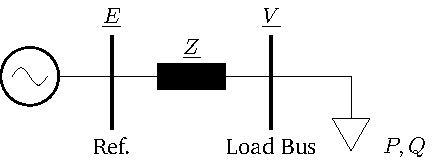
\includegraphics{./tikz_graphics/images/analytical_model.pdf}
    \caption[Simple load source system for deriving voltage power behaviors]{Simple load source system for deriving voltage power behaviors; own illustration after \autocite{machowski_2020,kundur_2022,milano_2010}}
    \label{fig:v-stability-system}
\end{figure}

When looking at the load flow equations, the transferable power over the system from bus one to bus two can be represented by
\begin{align}
    S&=P + jQ = \underline{V} \cdot \underline{I}^* \notag \\[12pt]
    &=\underline{V} \cdot \frac{\underline{E}^* - \underline{V}^*}{-jX} \notag \\[6pt]
    &=\frac{j}{X} (EV \cos \phi + jEV \sin \phi -V^2). \notag
\end{align}
These equations can be split up into the transferable real power in \autoref{eq:func-p-transfer} and the transferable reactive power in \autoref{eq:func-q-transfer}, which might be more common in knowledge and use.
\begin{align}
    P&=-\frac{EV}{X} \cdot \sin \phi \label{eq:func-p-transfer} \\[6pt]
    Q&=-\frac{V^2}{X} + \frac{EV}{X} \cdot \cos \phi \label{eq:func-q-transfer}
\end{align}
After elimination of $\phi$\footnote{due to the setpoint of the reference voltage}, a second order equation dependent on $V^2$ can be obtained.
Simplifying the terms and rearanging is giving the following \autoref{eq:transfer-func}.
\begin{align}
    &-P^2 - \frac{E^2}{X}Q + \bigg(\frac{E^2}{2X}\bigg)^2 \geq 0 \label{eq:transfer-func} \\[12pt]
    &P \leq \frac{E^2}{2X} \quad\text{for}\quad Q=0 \label{eq:simplified-transfer-p} \\[6pt]
    &Q \leq \frac{E^2}{4X} \quad\text{for}\quad P=0 \label{eq:simplified-transfer-q}
\end{align}
\sidenote{Power angle $\phi$ and its usage}
The easy intuitively accessed functions, which can be kept in mind are \autoref{eq:simplified-transfer-p} and \autoref{eq:simplified-transfer-q}.
These represent the functions of the voltage dependence on the real power, when setting the reacitve power to zero, and vice versa. 
This accounts for power factors of $\cos \phi = 0$ or respectively $\sin \phi = 0$, or translated to the angle itself $\phi = \{0^\circ; 90^\circ\}$.
\footnote{for all angles in the interval of $\phi = [0^\circ, 180^\circ]$}
One note to take here, is that the power factor is not consistently used.
For load flow calculations mostly the sine and cosine representation of the angle between current and voltage is used, for stability analysis, often the tangent function is preferred.
A table and plot comparison of relations between the functions $\cos$, $\sin$, and $\tan$ are included in the appendix \autoref{app:trogonometric-func-comp}. 
This also leads to the dependency of $\tan \phi$ in the plotting of the so called Nose Curves, the solutions of \autoref{eq:transfer-func}.

\begin{figure}[htbp!]
    \centering
    % \missingfigure{Nose Curves P and Q dependent on V}
    \begin{subfigure}[b]{.49\linewidth}
        \includegraphics[width=\linewidth]{development_files/theoretical/plots/p_v_analytical.pdf}
        \subcaption{P-V \glqq Nose Curve\grqq}
    \end{subfigure}
    \begin{subfigure}[b]{.49\linewidth}
        \includegraphics[width=\linewidth]{development_files/theoretical/plots/v_q_analytical.pdf}
        \subcaption{V-Q Curve}
    \end{subfigure}
    \caption[Power Voltage Curves resulting from maximum power transfer equations]{Power Voltage Curves resulting from maximum power transfer equations; Considering a Network impedance of $\underline{Z}=jX$ with $X=0.15\text{ p.u.}$ and a system base power of $S_\mathrm{sys;base}=2200\text{ MVA}$; Note, that $\arctan(0) = \arccos(1)$; own illustration after \autocite{machowski_2020,kundur_2022,cutsem_1998}}
    \label{fig:v-stability-system}
\end{figure}

\sidenote{What can one see and read from the curves?}
The typical nose shape is visible for a simple network, with only considering reactances $X$ as attributes of the line or transmission grid and a reference value at the reference bus set to $\underline{E}=1\angle0$ p.u.
Directly visible, that no static solution can be found, when surpassing a certain level of real power. 
This maximum often is referred to as the power transfer limit of the grid or network.
Aside from that there are two solutions possible for all the other values of the power smaller than the maximum power transfer limit.
On the other sidem when looking at the V-Q curve from \autoref{fig:v-stability-system} b), the first thing to notice is the inverted axis compared to the P-V curves.
This is a common practice, as the voltage is the more independent variable here \autocite{kundur_2022}.
Secondly the shape and the resulting values are different.
The Q-V curve can be understood as the reactive power support at the load bus.
One can obtain from the curve, that the values above the zero line account for a capacitive reactive power support, which is limited with the relation of \autoref{eq:simplified-transfer-q}.
The part in the negative region is related to an inductive support, due to the inductive nature of the transmission grids there is also no limit.
But what one can easily see is the continously increasing voltage in order to equalize the missing compensatiom \autocite{kundur_2022}.
When looking at the voltage of the maximum active power transfer, and reading the reactive power for that, one would see a positive, meaning capacitive reactive power support at the load bus.
This would be described as the natural power of the line, when fully compensating the reactances and operating the line with a solely ohmic resistance.
These curves can be also transfered in the three dimensional space, with the axis P-Q-V giving a full observation of static power voltage relations.

\subsection{Evaluation of Time Series Calculation}
\label{sec:stability-indices}

\sidenote{Basic idea\\and references}
The idea behind stability indices is monitoring the current voltage stability state of the power system in relation to the critical points or operational limits.
This applies not only to static load flow cases, but for time series calculations of short circuits, load shedding or other disturbances.
Reviewing possible indices, either for online resp. real time monitoring or for subsequent analysis after a simulation, is out of the scope of this thesis.
For static analysis, often the Jacobian Matrix is used as basis.
The Newton-Raphson algorithm for load flow analysis is based on this construct, as well as many indices.
Voltage stability can be mathematically formulated, if the Jacobian Matrix is not singular.

% \textcite{danish_2015} has already included an extensive review in his work, with reference to \textcite{doigcardet_2010}, which is focussing on indices trying to show remaining capabilites to the static power limit. 
% These indices are often referred to as a linearization of the static assessment with nose curves, as these simple power voltage illustrations have higly nonlinear behavior esp. around the critical point. 

\sidenote{Indices adressing numerical problems}
Using solely the signularity of the Jacobian Matrix for determination of a stable system is numerical hard to solve and usually very error-prone.
This problem leads to the necessity of applying other methods or indices for stability assessment. 
Further, the relation of the system state to the critical voltage collapse point is highly nonlinear in the Jacobian Matrix. 
This problem is adressed by the indices in various ways, leading to a more or less linearized relation \autocite{machowski_2020,danish_2015}. 
\textcite{danish_2015} is proposing indices, that are also based on the Jacobian Matrix, and shows comparitive characteristics between Jacobian Matrix and system variable based voltage stability indices. 
% These Jacobian Matrix based indices are listed and shortly described in \autoref{app:jacobian-voltage-indices}, while the comparative characteristics are described in \autoref{app:jacobian-vs-system-indices}. 
The aforeside mentioned work of \textcite{doigcardet_2010} is focussing on these indices in particular.
This thesis is thus not considering these static assessment based indices, as the simulative nature allows for easier static eavluation with simple nose curves. 

\sidenote{Comparability of time series}
Considering the nose curve from \autoref{fig:v-stability-system}, one can see a static solution around the maximum power transfer, that is way below the initial voltage.
And when taking into account grid codes and their connection rules for generation units, also outside any \ac{FRT} behavior neither a static reasonable operation point.
Therefore, not only to comply with grid codes, but to avoid operational unit failures due to high currents or high voltages, this \acs{FRT} behavior shall be used as a sort of envelope.
This allows or easy comparison, either if the scenario is exceeding this grid code envelopes seen as critical, but also to calculate the significance of this violation.
\textcite{scheiner_2022} and \textcite{wildenhues_2015} propose an index called \ac{TVI}
The index is, simplified summarized, integrating the envelope violation over the simulation time.
Although they are using not \acs{FRT} curves, but a more scientific representation of such an envelope, this idea shall be implemented and used in this thesis.

\sidenote{Description of the Index}
The mathematical background shall be introduced in the following.
First, the envelopes are computed according to \autoref{eq:t-low} and \autoref{eq:t-upp}.
The typical used values for this envelope are $v_\mathrm{st}=0.9$ and $\beta \in [0.05,0.1]$ according to \textcite{wildenhues_2015}.
If one wants to choose the \acs{FRT} curves as envelopes, the technical connection guide lines describe these curves for different generation units connected to different voltage level grids \autocite{vde-tar_2018,vde-tar_2023}.
\begin{align}
    T_\mathrm{low}(t) &= \frac{\bigg(\frac{t}{t_\mathrm{end}} \cdot \exp(\frac{t}{t_\mathrm{end}})\bigg)^\beta}{\exp(\beta)},\quad \forall t \in [t_\mathrm{f}, t_\mathrm{end}] \label{eq:t-low} \\[12pt]
    T_\mathrm{upp}(t) &= 2-T_\mathrm{low}(t) \label{eq:t-upp}
\end{align}
The integral is then calculated as the difference between the voltage magnitude and the envelope boarder, resp. the area between the two curves exceeding the envelope.
The voltage difference equates the voltage violation in \autoref{eq:tvi}.
This is achieved through the case dependent function in \autoref{eq:tvi-integration-rules}.
\begin{align}
    \text{TVI} &= \int_{t_\mathrm{f}}^{t_\mathrm{end}} v_\mathrm{v}(t) \dd{t} \label{eq:tvi}\\[12pt]
    v_\mathrm{v}(t) &= \begin{cases}
            T_\mathrm{low}(t) - v(t) & \text{if } v(t) < T_\mathrm{low}(t)\\
            v(t) - T_\mathrm{upp}(t) & \text{if } v(t) > T_\mathrm{low}(t)\\
            0 & \text{otherwise}
    \end{cases} \label{eq:tvi-integration-rules}
\end{align}
As this index is dependent on one voltage value, measurement is typically done at each bus.
The \acs{TVI} then is calculated for every bus.
One can calculate the \acs{TVI} for the total system according to \autoref{eq:tvi-system}.
It can be understood as the envelope violation magnitude multiplied by the time.
\begin{align}
    \text{TVI}_\mathrm{tot} &= \sum_{i \in N_\mathrm{busses}} \text{TVI}_i \label{eq:tvi-system} \\[12pt]
    \text{CSI} &= \frac{1}{N_\mathrm{busses}} \sum_{i=1}^{N_\mathrm{busses}} \text{TVI}_i \label{eq:csi-system}
\end{align}
On the other hand one can calculate the \ac{CSI} with help of the \acs{TVI} as displayed in \autoref{eq:csi-system}.
This index is not only giving an approach to normalization the \acs{TVI} regarding to grid sizes through the total number of busses $N_\mathrm{busses}$.
With this index, short circuit scenarios and their dynamic affecct on various grids can be compared.
On the other hand it could be used as an average and related to the bus individual \acsp{TVI}.
This allows for evaluation of the most affected bus(ses) in the system.

%%%%%%%%%%%%%%%%%%%%%%%%%%%%%%%
\section{Power System Modeling}

The simulation of power systems is a crucial tool, not only for stability studies, but for evaluating extensions or modifications in the planning process, the development of assistance systems for operational management, and many other applications. \quelle 
Due to the complexity of the systems, simulations are often simplified. 
Not only with model constraints, but as well in the way of calculations. 
Mainly seperating between \acf{EMT} and \acf{RMS} simulations, the latter is used in this thesis. 
The \autoref{app:power-system-modeling} is giving more details, literature, and summarizing the processes behind the used tool \textit{diffpssi}, if the reader is further interested in the topic.

\subsection{Transformer Electric Model and Behavior}
\label{sec:trafo-model}

% \begin{figure}[htb!]
%     \centering
%     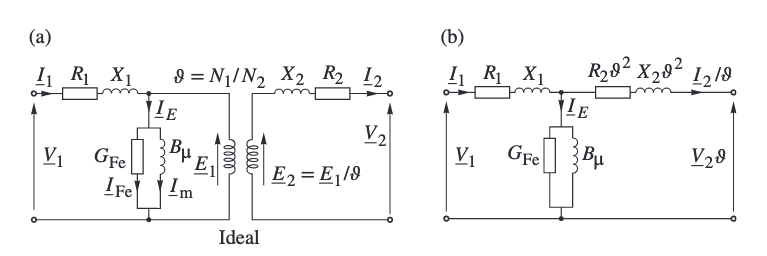
\includegraphics[width=.8\textwidth]{fundamentals/trafo_model_deviation.png}
%     \caption[Two-Winding Transformer Circuit in the Positive Sequence]{Two-Winding Transformer Circuit in the Positive Sequence; a) ideal representation with impedances on each \acs{HV} and \acs{LV} side and b) related impedances on the XX side; own figure after \autocite{machowski_2020}}
%     \label{fig:trafo-model-deviation}
% \end{figure}

% \sidenote{Basics}
Typical for \acs{RMS}-modeling is the usage of sequence components, especially the positive sequence for symmetrical grid operation and test cases. \quelle 
An equivalent circuit for the positive sequence is shown in \autoref{fig:trafo-model} part a), respectively reduced to the transformer ratio, the series impedances of the windings on the \acs{LV} and \acs{HV} side, and the shunt branch affected by iron and magnetization losses. \autocite{machowski_2020,kundur_2022,milano_2010}

The transformer ratio is typically noted as $\underline{\vartheta}$. 
Generally speaking it is the ratio between the number of windings of the secondary side to the primary side, as noted in \autoref{eq:trafo-ratio-easy}. 
With the typically used calculation unit \glqq per unit\grqq\footnote{means standardization to a reference value; further information on page \pageref{chap:symbols} and \textcite{machowski_2020}, Appendix A}, the ratio becomes one in the standard case. 
A transformer ratio, which is only shifting current angles with the shifting angle $\phi$, is represented through a complex number using the Euler Identity, as shown in \autoref{eq:trafo-ratio}.
\begin{align}
    \vartheta&=\frac{N_2}{N_1} \label{eq:trafo-ratio-easy} \\[6pt]
    \underline{\vartheta}&=\frac{N_2}{N_1} \cdot \exp(j \cdot \phi \cdot \frac{\pi}{180})\label{eq:trafo-ratio}
\end{align}

\begin{figure}% [htb!]
    \centering
    % \captionsetup[subfigure]{justification=centering} 
    \begin{subfigure}[c]{.53\textwidth}
        \centering
        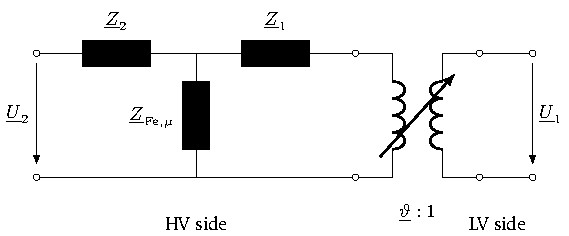
\includegraphics[width=\linewidth]{tikz_graphics/images/transformer_complete.pdf}
        \subcaption{Ideal Representation}
    \end{subfigure}
    \begin{subfigure}[c]{.46\textwidth}
        \centering
        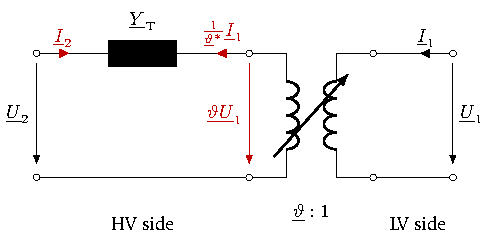
\includegraphics[width=\linewidth]{tikz_graphics/images/transformer_reduced.pdf}
        \subcaption{Simplifyied Representation}
    \end{subfigure}
    % 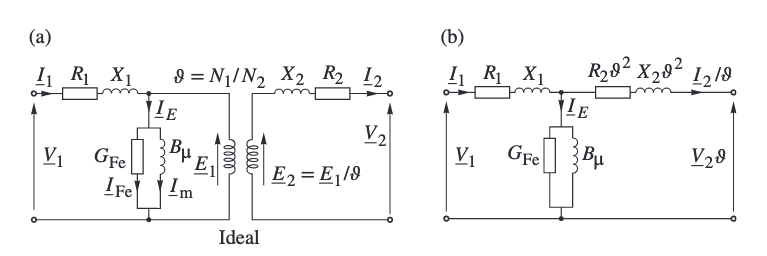
\includegraphics[width=.8\textwidth]{fundamentals/trafo_model_deviation.png}
    \caption[Two-Winding Transformer Circuit in the Positive Sequence]{Two-Winding Transformer Circuit in the Positive Sequence; a) ideal representation with impedances on the \acs{HV} side and b) simplifyied circuit with only the series impedance related on the \acs{HV} side; own figure after \autocite{machowski_2020,kundur_2022,milano_2010}}
    \label{fig:trafo-model}
\end{figure}

\sidenote{Simplifications}
The first simplification is step is considering two assumptions. 
First, the iron and magnetization losses are neglectable. 
This can be illustrated with a short-circuit test of the transformer on the secondary side. 
During this test, one can obtain with the concept of a voltage devider, that
\begin{align}
    \underline{U}_\mathrm{Fe, \mu} \ll \underline{U}_\mathrm{T,rated}, \notag
\end{align}
meaning that the shunt branch impedance is much greater that the series impedance of the transformer. 
Secondly, it is assumed, that the on the primary side related impedance of the secondary side, is equal to the impedance on the primary side. 
This leads to a symmetrical circuit of the transformer and the positive sequence equivalent circuit simplifies to \autoref{fig:trafo-model} part b). 
Mathematically this is shortly expressable as \autoref{eq:related-impedances}, \autoref{eq:trafo-symmetrical}, and \autoref{eq:series-impedance}. \autocite{machowski_2020,kundur_2022,milano_2010}
\begin{align}
    \underline{Z}_1 &= R_1 + jX_1\text{;}\quad\underline{Z}_2 = R_2 \vartheta^2 + jX_2 \vartheta^2 \label{eq:related-impedances} \\
    \underline{Z}_1 &= \underline{Z}_2 \label{eq:trafo-symmetrical} \\
    \underline{Z}_\mathrm{T} &= \underline{Z}_1 + \underline{Z}_2 \label{eq:series-impedance}
\end{align}
The afore described simplification leads to only the necessity of considering the series impedance. 
Considering the afore mentioned normal ratio of $\vartheta=1$ in the per unit system, the Python framework \textit{diffpssi} has been using this model with only the series impedance and no variable ratio, meaning no shunt branches, before.

\sidenote{Introducing variable transformer ratios}
When one wants to look at variable transformer ratios, either with representing vector groups, or implementing \acfp{OLTC}, this model of only considering the series impedance has to be extended. 
Using shunt branches, the variable ratio behavior can be represented in a $\Pi$-model, as shown in \autoref{fig:pi-transformer}. \autocite{machowski_2020,kundur_2022,milano_2010}

\begin{figure}%[htb!]
    \centering
    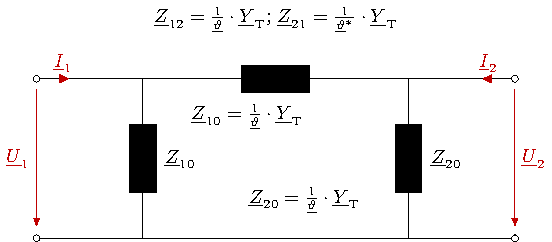
\includegraphics[width=.7\textwidth]{tikz_graphics/images/transformer_pi.pdf}
    \caption[$\Pi$-representative circuit of an idealized transformer with a tap changer]{$\Pi$-representative circuit of an idealized transformer with a tap changer; own figure after \autocite{milano_2010,burlakin_2024}}
    \label{fig:pi-transformer}
\end{figure}

Looking at the transformer as a black box two-port, with the index one being the \ac{LV} side, the index two being the \ac{HV} side, the admittance matrix for the variable ratio behavior can be expressed as in \autoref{eq:admittance-behavior}. 
The voltages and current are defined as in \autoref{fig:trafo-model} part b). 
With rearranging the equation, one can obtain the admittance matrix of the $\Pi$-model with to the \acs{HV} side related values as in \autoref{eq:admittance-matrix-pi}. \autocite{milano_2010,burlakin_2024}

\begin{align}
    \begin{bmatrix}
        \underline{I}_1 \\ {\color{ees_green}\underline{\vartheta}^*} \underline{I}_2
    \end{bmatrix}&= 
    \begin{bmatrix}
        \underline{Y}_\mathrm{T} & -\underline{Y}_\mathrm{T} \\
        -\underline{Y}_\mathrm{T} & \underline{Y}_\mathrm{T}
    \end{bmatrix} \cdot
    \begin{bmatrix}
        \underline{U}_1 \\ {\color{ees_green}\frac{1}{\underline{\vartheta}}}~\underline{U}_2
    \end{bmatrix} \label{eq:admittance-behavior} \\[12pt]
    \underline{\mab{Y}}_\mathrm{\Pi,T}&=\underline{Y}_\mathrm{T} \cdot
    \begin{bmatrix}
        1 & -\frac{1}{\underline{\vartheta}} \\
        -\frac{1}{\underline{\vartheta}^*} & \frac{1}{\underline{\vartheta}\underline{\vartheta}^*} 
    \end{bmatrix} \label{eq:admittance-matrix-pi}
\end{align}

For calculation of the individual shunt branches, one can apply the standard representation of two-ports consistent of a linear $\Pi$-circuit:
\begin{align}
    \begin{bmatrix}
        \underline{I}_1 \\ \underline{I}_2
    \end{bmatrix}=
    \begin{bmatrix}
        \underline{Y}_{10} + \underline{Y}_{12}& -\underline{Y}_{12} \\
        -\underline{Y}_{21} & \underline{Y}_{20} + \underline{Y}_{21}
    \end{bmatrix} \cdot
    \begin{bmatrix}
        \underline{U}_1 \\ \underline{U}_2
    \end{bmatrix} \notag % \label{eq:shunt-calc}
\end{align}
When equating this with \autoref{eq:admittance-matrix-pi}, the shunt branches can be calculated respectivly giving the admittances written down as \autoref{eq:y-12}, \autoref{eq:y-10}, and \autoref{eq:y-20}, as they are noted in \autoref{fig:pi-transformer} as well. \autocite{milano_2010,burlakin_2024}
\begin{align}
    \underline{Y}_{12}&=\frac{1}{\underline{\vartheta} \cdot \underline{a}_\mathrm{T}} \cdot \underline{Y}_\mathrm{T} \notag \\[6pt]
    \underline{Y}_{21}&=\frac{1}{\underline{\vartheta} \cdot \underline{a}_\mathrm{T}^*} \cdot \underline{Y}_\mathrm{T}\text{, and} \label{eq:y-12} \\[12pt]
    \underline{Y}_{10}&=\bigg(1 - \frac{1}{\underline{\vartheta} \cdot \underline{a}_\mathrm{T}}\bigg) \cdot \underline{Y}_\mathrm{T} \label{eq:y-10} \\[12pt]
    \underline{Y}_{20}&=\frac{1}{\underline{\vartheta}} \cdot \bigg(\frac{1}{\underline{\vartheta}} - \frac{1}{\underline{a}_\mathrm{T}}\bigg) \cdot \underline{Y}_\mathrm{T} \label{eq:y-20} 
\end{align}

\sidenote{Per unit system\\specialities}
Reactances and resistances are referred to the base voltage and apparent power of the operational unit, such as the transformer. 
The power system simulation uses its own base voltage and base apparent power, enabling the use of one single calculation domain. 
This is done to simplify the calculation and to make the results easily comparable to each other. 
Hence, the reffered values have to be transformed from the equipment based values to the simulation based values. 
The relation for the transformer admittance is defined as follows. 
Generally speaking, this thesis is using and reffering to the per unit based values, although it is not denoted in the index of the values.
\begin{align}
    \underline{Y}_\mathrm{T,~based}&=\underline{Y}_\mathrm{T} \cdot \frac{S_\mathrm{n}}{S_\mathrm{n,~sim}} \label{eq:y-t-based} \\[6pt]
    \underline{Z}_\mathrm{line,~based}&=\underline{Z}_\mathrm{line} \cdot \frac{S_\mathrm{n,~sim}}{V_\mathrm{n,~sim}^2} \label{eq:y-line-based}
\end{align}
Displayed like in \autoref{eq:y-t-based}, the characteristic of the operational unit is referred to the simulation base value. 
Here, the admittance of the transformer is multiplied with its own rated apparent power, then devided by the apparent power of the simulation system. 
Similar, the impedance of the lines are calculated via \autoref{eq:y-line-based}. 
This specialities are considered in the tap changer modeling, thus further information is given by \textcite{machowski_2020}, Appendix A.
Additionally, \textcite{glover_2017a} are giving some transformer specific calcualtions and examples in chapter 3.3.

\subsection{Further Considerations of a Transformer Model}
\label{sec:further-considerations}
\mycomment[MK]{Ist die section überhaupt relevant? Eigentlich könnte man ja auch denken, dass die etwas überflüssig ist...}

The following described (possible) characteristics of transformers shall not be considered in this thesis.
They are mentioned in case differences towards other simulation tools occur, which might consider these.
However, they could be also seen as possible extension of this thesis.
Some of them could target the stabilization of voltage instable scenarios better, e.g. phase shifting transformers. 
All of the following is a synthesis of different standard literature, but esp. \autocite{schwab_2022,oeding_2016,machowski_2020,kundur_2022}.

\sidenote{Vector Groups}
The first consideration are so called vector groups.
These represent a different internal interconnection scheme and are thus resulting in a different magnetic coupling of the single phase windings.
Under the consideration of different treatment as star, delta or mixtures of them, the ratio is not only phase shifted, but can as well be differing by the factor $\sqrt{3}$. 
Relevant for the modeling is only the resulting phase rotation, as length, star or delta consideration or else is not changing the overall ratio of the transformer.
The relevant ratio is dependent on the grid, the suitable transformer is then chosen after that.

\begin{figure}[htb!]
        \centering
        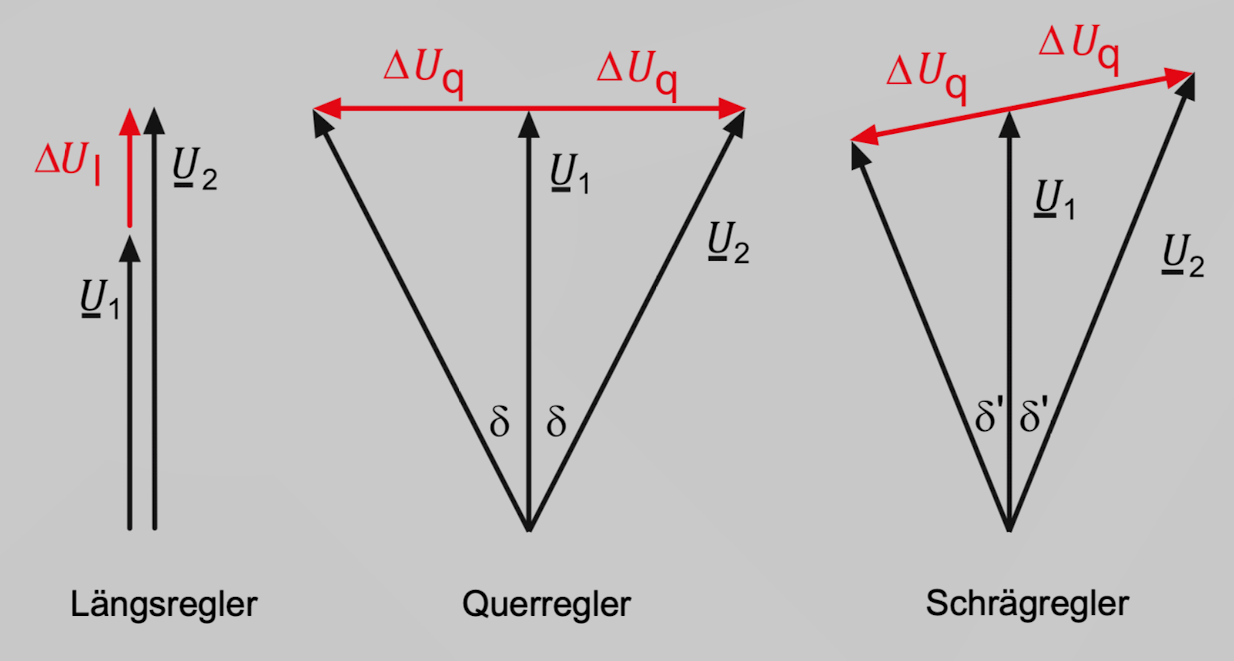
\includegraphics[width=.9\linewidth]{modeling/transformer_controls.png}
        \caption[Illustration of the voltage vectors for different regulating transformers]{Illustration of the voltage vectors for different regulating transformers; after \autocite{schwab_2022}}
        \label{fig:regulating-transformer-types}
\end{figure}

\sidenote{Regulating transformers}
When looking at regulatable transformers, there are three main types, as depicted in \autoref{fig:regulating-transformer-types}.
In this thesis only the simplest case, the longitudinal controlled transformer type is relevant and modeled. 
It is only capable of varying the voltage magnitude.
The remaining two are either just regulating and changing the phase angle, and therefore the imaginary part of the voltage, or a mixture of the both first described.
Important to note on the behalf of voltage stability is, that the longitudinal controller cannot actively control the reactive power, and thus act directly on the voltage stability.
It can only influence the voltage and thus hold the bus or brach longer in a certain defined voltage band.

\subsection{Use of Power System Simulation Tools}
\label{sec:simulation-tools}

\sidenote{diffpssi}
For this thesis relevant are mainly two Power System Simulation tools.
The first and main objective, \textit{diffpssi} is an open source project from Georg Kordowich, member of the chair hosting this thesis.
This open source tool provides a \acs{RMS} domain simulation of Power Systems, considering passive grid elements like lines, shunts, loads etc., but dynamic and controlled models like Synchronous Machines, Inverters or similar as well.
The project and the integration of a full Synchronous Machine model is presented in the published paper of \textcite{kordowich_2023}.
The project is based on dependencies like numpy, but can as well use the Python module \textit{PyTorch} as backend.
\textit{PyTorch} allows the differentiation of simulation variables.
With this, optimzation of grid and machine parameters is possible.
Future extension and usage in the topics like voltage stability and resp. or control strategies is likely as well.

\sidenote{DIgSILENT PowerFactory}
The second relevant tool is a commercial software called \textit{PowerFactory} by the company \textit{DIgSILENT}.
Modeling of the power system elements is described in its technical references, but not open source like \textit{diffpssi}.
In this thesis it is used as comparative tool, as it is also widely used in companies and at universities for power system studies and research.
The accounted version is \textit{DIgSILENT PowerFactory 2023 SP1}.

\sidenote{Other open source tools}
To give an overview of other open source power system simulation projects, one can have a look at \href{https://github.com/ps-wiki/best-of-ps}{this GitHub repository}.
At the submission date of this thesis, this repository is getting updated on a regular basis.
\textcite{jinningwang_2025} ranks around 140 open-source projects for power system analysis, grouped into 15 categories.
If one wants to compare, investigate or look out for other funcitonalities, modeling techniques or software structures, this can be used as a starting point.
        
%%%%%%%%%%%%%%%%%%%%%%%%%%%%%%%
\section{On-Load Tap Changer Controls}

Regarding the planned specific evaluation of \acs{OLTC} controls, this part of the Fundamentals section aims to clarify the status on current used control methods.
Further, it describes the done advancements regarding the addition of a \acf{FSM}.
For readers, that are not familiar with this module, it is quickly introduced, and the currently available control scheme is briefly described.

\subsection{Commonly Used On-Load Tap Changer Control}

A few basics are of interest for understanding differences between real world behavior, or possible ways of building up an \acs{OLTC} transformer control. 
This control theory difference can be limiting as well for the results and objectives compared to the actual possible control in the field.

% \subsubsection{Typical presets are manually set}
\sidenote{Typical presets are manually set}
The target voltage is typically set from the control room of the grid operator, coming from pre-calculated load flow analysis. 
This can be set hours before, or even day-ahead with the estimated loads of the grid. 
This value is set locally for each operating unit subsequently. 
The control is then operating locally and without further involvement of the grid operator. \quelle

% \subsubsection{Discrete controllers are used in the field}
\sidenote{Discrete controllers are used in the field}
Typically the used controller in the field is a discrete controller, which can change tap positions under load within a time frame of around a few seconds. 
Practical tap steps are around $2~\mathrm{\%}$ of the overall transforming ratio. 
The control is set up with a dead band, to avoid unnecessary tap changes. 
It is necessecary to note here, that this control and its mathematical caracteristics contains logical elements, blocks, and delays, which cannot be translated in a typical control theory transmission function. 
This leads to the missing possibility to easily obtain mathematical stability for the control of the overall considered power system. \autocite{machowski_2020,kundur_2022}

\subsection{Advancement: Fast Switching Module and its Control}
\label{sec:fsm-description}

\begin{wrapfigure}[18]{L}{0.5\linewidth} 
    \centering
    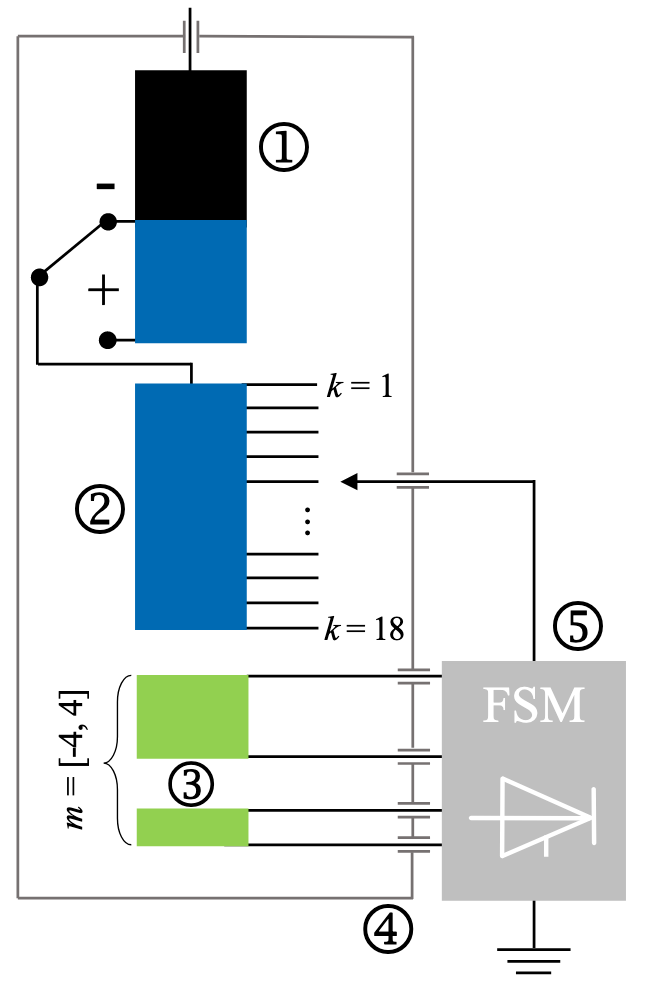
\includegraphics[width=.77\linewidth]{fundamentals/scheme_fsm.png}
    \caption[Schematic illustration of the \acs{FSM}]{Schematic illustration of the \acs{FSM}; from \autocite{burlakin_2024a}}
    \label{fig:phys-scheme-fsm}
\end{wrapfigure}
\sidenote{Physical funcitonalities}
The basic idea of the \acf{FSM} is using a conventional \acs{OLTC}, but connecting it with a power electronics based additional switching unit.
The complete module and a detailed description can be found in \autocite{burlakin_2024a} and \autocite{maschinenfabrikreinhausengmbh_2023}.
This module is serial to the normal tap changer, and can connect resp. make use of additional windings, either as addition or subtraction.
This module can be used in any tap position of the \acs{OLTC}.
The \acs{FSM} windings have to be located on the same core as the main and \acs{OLTC} regulating windings.
In contrast to the conventional \acs{OLTC} not only the next lower or higher tap position can be accessed.
Instead each \acs{FSM} tap position is reachable from every other, inroducing much bigger possible switching steps at one time.
The tap increment $\Delta m$ of the \acs{FSM} is understood as factor of the conventional tap increment.
Typically used values for $\Delta m$ are $1$ or $2$, the number of tap positions is limited in the interval $[-4,4]$.
Considering a \acs{OLTC} voltage change of $0.02$ p.u. per tap, this is resulting in a maximum change magnitude of $32$ \%.
With a minimum time constant of $0.02$ s\footnote{limited by the filtering of a $50$ Hz signal}, this results in possibly large dynamic actions.
A scheme of the structure is added in \autoref{fig:phys-scheme-fsm}, where following items are numbered:
\begin{enumerate}[label=\protect\circled{\arabic*}]
    \item \textbf{Main winding} with coarse change-over selector
    \item \textbf{Regulating winding} for the \acs{OLTC}
    \item \textbf{Regulating winding} for the \acs{FSM}
    \item \textbf{Tank} for the reactor
    \item \textbf{\acs{FSM}} in a seperate container
\end{enumerate}

\sidenote{FSM control scheme}
Going further into the grid relevant aspects, the operational control of this extended transformer, \textcite{burlakin_2024} gives a first approach for a control scheme.
This is based on the conventional understanding and control of \acsp{OLTC} so far.
The control loop can be observed in \autoref{fig:fsm-control-loop}.
It is also implemented in the comparative tool \textit{DIgSILENT PowerFactory}, just with one slight modification.
The \acs{OLTC} is not only activated after the \acs{FSM} reached an extreme position, thus the last is not preferred for switching.
The control enables the \acs{OLTC} first when exceeding the deadband.
The \acs{FSM} is only getting activated, when the function for tap skipping is not zero anymore.

\begin{figure}[htb!]
    \centering
    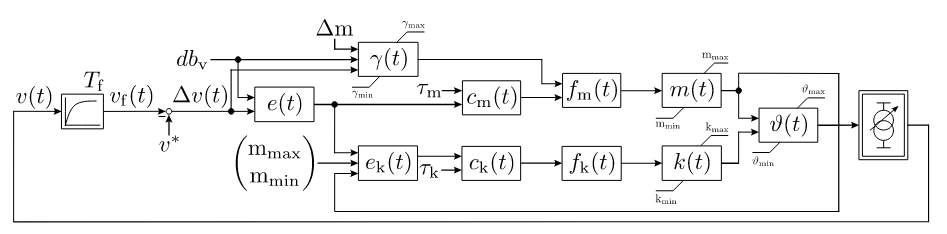
\includegraphics[width=\textwidth]{modeling/fsm_control_scheme.png}
    \caption[Control loop of a \acf{FSM}]{Control loop of a \acs{FSM}; scheme based on \textcite{burlakin_2024}}
    \label{fig:fsm-control-loop}
\end{figure}

\sidenote{Details of the control circuit}
Generally speaking, the control scheme is devided into two paths, the \acs{FSM} and the \acs{OLTC} part.
The control scheme input $v_\mathrm{f}$ is the measurement delayed or filtered voltage at the decided bus.
Filtering is represented by a PT1 block with the filtering time constant $T_\mathrm{f}$.
Subtracted from the reference voltage $v^*$ this is the voltage deviation, which is in the interest of the tap changer. 
If the absolute voltage difference $\Delta v$ is bigger than the the deadband of the control, the function $e(t)$ is enabling the cascaded memory function $c_\mathrm{m}(t)$, and for the \acs{OLTC} path $e_\mathrm{k}(t)$.
In the depicted scheme in \autoref{fig:fsm-control-loop} from \autocite{burlakin_2024} the \acs{OLTC} is only activated, if the \acs{FSM} is in one of its end positions.
Subsequently, the function $c_\mathrm{k}(t)$ is the memory function for the \acs{OLTC}, both with their specific time constants $\tau_\mathrm{m}$ resp. $\tau_\mathrm{k}$.
The functions $f(t)$ are determing the tap change, which is applied to the respective tap position functions $m(t)$ and $k(t)$, with other words they are the derivatives.
For the \acs{OLTC}, this tap change function $f_\mathrm{k}(t)$ can have values $\in [-1,1]$ as output, while for the \acs{FSM} function $f_\mathrm{m}(t) \in [\gamma_\mathrm{min},\gamma_\mathrm{max}]$ can be formulated.
The amount of tap changes for the \acs{FSM} is calculated through the function $\gamma(t)$, which embeddes the tap skipping function $\eta(t)$.
Together they define the tap change input as described in \autoref{eq:tap-skip} and \autoref{eq:gamma}
\begin{align}
    \eta(t) &= \text{floor}\bigg( \frac{\vert \Delta v(t) \vert}{db_\mathrm{v} \cdot \Delta m} \bigg) \label{eq:tap-skip}\\[12pt]
    \gamma(t) &= \begin{cases}
        \gamma_\mathrm{max} & \text{if } \eta(t) > \gamma_\mathrm{max} \\
        \gamma_\mathrm{min} & \text{if } \eta(t) < \gamma_\mathrm{min} \\
        \eta(t) & \text{otherwise}
    \end{cases} \label{eq:gamma} \\[6pt]
    \text{for}\quad&\eta(t),\gamma(t) \in \mathbb{Z} \notag
\end{align}
Lastly, the transformer ratio dependent on the time step is formulated as 
\begin{align}
    \vartheta(t) = \begin{cases}
        \vartheta_\mathrm{max} & \text{if }\vartheta > \vartheta_\mathrm{max} \\
        \vartheta_\mathrm{min} & \text{if }\vartheta < \vartheta_\mathrm{min} \\
        \vartheta_0 + \Delta v (k(t)-k_0+m(t) \cdot \Delta m) & \text{otherwise.}
    \end{cases}\label{eq:fsm-control-transformer-ratio}
\end{align}
A more detailed description is given by \textcite{burlakin_2024}, where standard values and their impact for the variables are described as well.

%%%%%%%%%%%%%%%%%%%%%%%%%%%%%%%
\section{Summary in Short and Simple Terms}

The fundamentals chapter introduced resp. showed resources for understanding the basics of voltage satbility, espacially considering the \acs{OLTC}.
An analytical derivation of power voltage characteristics in grid calculations has been introduced with the Nose Curve examplary for a simple system.
A suitable index is proposed for comparing \ac{TDS} dynamics of different scenarios with the \acf{TVI}.

The mathematical description of a variable ratio transformer is derived, further possible applications and imrpvements illustrated.
The in this thesis used power system simulation tools were introduced and a reference given, where a few open-source tools are compared.
Lastly, the new advancement regarding the \acs{FSM} and its control proposal is described.``

% \commenting{
%     Shortly summarize the bullet points / key takeaways from the topics
%     \begin{itemize}
%         \item Voltage Stability - Static and dynamic
%         \item Power System Modeling - especially Transformer Modeling
%         \item New Advancement from Ilya
%     \end{itemize}
% }